\subsection{データの収集}
\label{sec_data_collection}

本研究では，ファインバブル（Fine Bubble，FB）発生装置 FBG-OS Type1 を用いてファインバブルを生成した．
実験系の概略を図\ref{fig_procedure}に示す．
酸素ボンベから供給される酸素と純水を HPLC ポンプおよび Air-Water Mixer で混合し，Dissolution Tubing を通過させて溶解槽に導入する．
溶解した気液混合流体は Discharge Tubing および Back Pressure Regulator を経て水温 30\,\textcelsius に保たれた Water Bath 内へ吐出され，FB 懸濁液として回収される．
回収した FB 懸濁液は 3-way stopcock を介して分取され，一部は Syringe Pump によって供給される純水を background として NanoSight LM10 に導入しナノバブル（Nanobubble，NB）濃度を測定した．
本稿では，NB の普及した呼称である UFB を用いて UFB 濃度（UFB conc.）と表記する．
また，別経路で PartAn SI にも導入し MB 濃度（MB conc.）を測定した．
生成された FB を含む水中の溶存酸素量（Oxygen content，Oxygen cont.）は Oxygraph により測定した．

本研究では，FB の生成条件を説明変数，生成された FB の物性値を目的変数として扱う．
ここで，説明変数とは目的変数を予測するために用いる変数であり，目的変数とは予測の対象となる変数である．

説明変数として設定した 6 つの因子とその設定水準を表\ref{tab_conditions}(A)に，本稿で扱う目的変数とその意味を表\ref{tab_conditions}(B)に示す．
これら 6 つの因子の組み合わせのうち 39 通りの操作条件について FB を生成し，各条件につき 1〜5 回の反復測定を行った結果，合計 82 サンプルのデータセットを構築した．
目的変数としては，UFB 濃度，MB 濃度，酸素含量に加えて，Mean size，Mode size，Size (bin) の計 6 種を測定したが，本稿で分析対象とする目的変数の選定については\ref{sec_condition}節で述べる．

\begin{table}[H]
    \caption{実験条件および目的変数の一覧}
    \vspace{2mm}
    \centering
    \begin{subtable}[t]{\linewidth}
        \centering
        \caption{説明変数と設定水準}
        \begin{tabular}{cc}
            \hline
            説明変数 & 設定水準 \\
            \hline
            溶解管長さ（Dissolve tube） & 0.12，2\,m \\
            溶解圧力（Dissolution pressure） & 2，3，4\,MPa \\
            吐出管長さ（Discharge tube） & 0.7，2，4，5\,m \\
            酸素流量（Flow speed (oxygen)） & 3.3，5，10，25\,mL/min \\
            水流量（Flow speed (water)） & 25，40，45，46.7\,mL/min \\
            水量（Water volume） & 50，100\,mL \\
            \hline
        \end{tabular}
        \label{tab_conditions_a}
    \end{subtable}

    \vspace{3mm}

    \begin{subtable}[t]{\linewidth}
        \centering
        \caption{目的変数とその意味}
        \begin{tabular}{cc}
            \hline
            目的変数 & 意味 \\
            \hline
            MB conc. & PartAn SI により測定した MB（Micro Bubble）濃度 \\
            UFB conc. & NanoSight LM10 により測定したナノバブル（Nanobubble）濃度 \\
            Oxygen cont. & Oxygraph により測定した溶存酸素量 \\
            \hline
        \end{tabular}
        \label{tab_conditions_b}
    \end{subtable}
    \label{tab_conditions}
\end{table}

\begin{figure}[H]
    \centering
    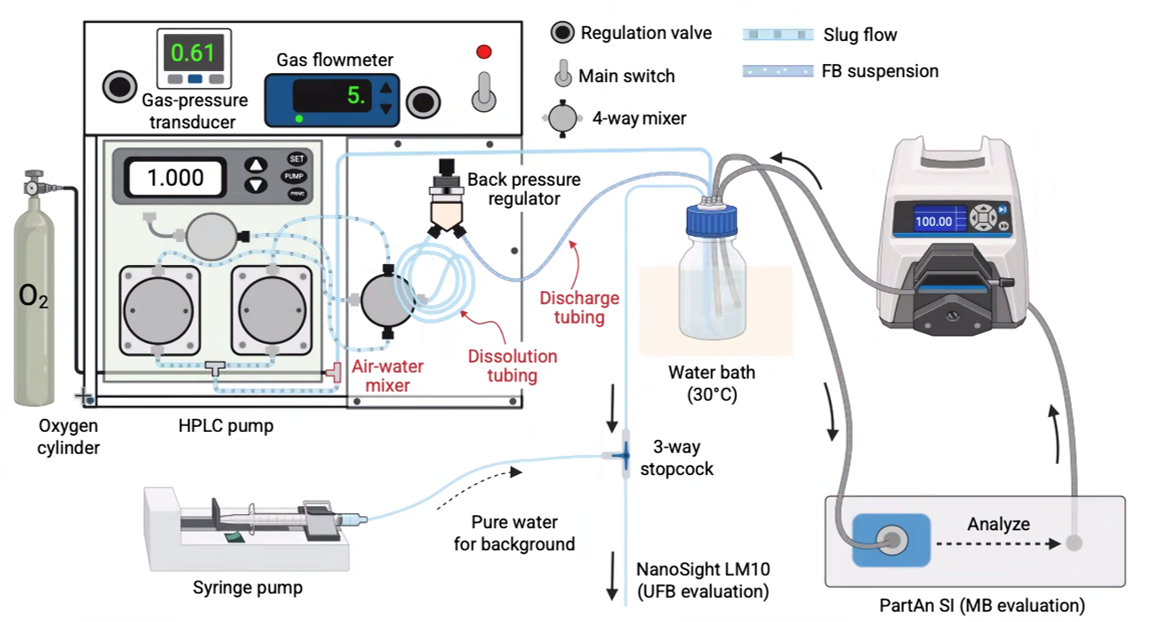
\includegraphics[width=0.7\linewidth]{figures/figure1_experimental_procedure.png}
    \caption{FB 発生・評価系の概略図}
    \label{fig_procedure}
\end{figure}
